\chapter{熱史、最後散射與原始湯}

\lectureoverview{宇宙的膨脹史也是一部熱史。我們先透過平衡來定義溫度，再透過散射來定義平衡。自由電荷使光子氣體維持熱化，形成普朗克譜；電子與質子結合時，輻射便退耦，但每個波長都隨尺度因子拉長，因此仍保有黑體形狀。光子與物質之間極大的數量比，解釋了為何復合發生時的溫度遠低於氫的電離溫度。繼續回溯，我們會依序經過最後散射、物質--輻射相等、電子--正電子對平衡，最後到達湮滅後留下的微小物質--反物質不對稱。}

\section{從模型擬合到熱史}

宇宙學模型至少由尺度因子的演化史與空間幾何指定，
\begin{equation}
a(t),
\qquad
k\in\{+1,0,-1\}.
\end{equation}
實際上，我們會先選定模型，計算其預測，再將預測與資料比較並調整參數。也可以直接從資料反向推論，但這種做法往往較不透明。

要從相對鄰近的天體判定曲率並不容易。就像在短距離的地表基線上，地球曲率只造成微小修正；宇宙學基線不夠長時，空間曲率的效應也很弱。這既是缺點，也是優點：一般的天體巡天無法精確判定\(k\)，但\(k\)即使存在中等程度的不確定性，也不妨礙我們有用地重建膨脹史。

兩類觀測量提供了大部分資訊。標準燭光給出亮度隨紅移的變化，天體巡天則給出各紅移區間內的天體數量。由此得到的擬合結果偏向具有顯著真空能貢獻的膨脹史。若要精確掌握曲率，就需要宇宙微波背景所提供、長得多的幾何基線。

現在我們轉而探討另一個問題。我們不再只問\(a(t)\)如何演化，也要問宇宙的溫度如何演化。這個問題得從一個更基本的問題開始：系統在什麼條件下才具有溫度？

\section{宇宙何時具有溫度}

溫度是熱平衡的性質。粒子集合透過碰撞趨近平衡，而碰撞必須比宏觀環境變化得更快。在膨脹宇宙中，有用的比較是
\begin{equation}
\tau_{\rm scatt}\ll H^{-1},
\label{eq:c07-equilibrium-condition}
\end{equation}
其中\(\tau_{\rm scatt}\)是特徵散射時間，\(H^{-1}\)是膨脹時間。若這個不等式不成立，宇宙的變化就會快於碰撞恢復平衡的速度。

想像一個完全反射的盒子。將一束雷射脈衝射入盒中，關上開口，並假設盒內只有光子。脈衝會無止盡地來回反射，但一般低能光子彼此散射的機率極低。光靠反射無法重新分配光子的能量，使其形成熱譜。因此，光子氣體不會只因受限於盒中就達到熱化。

自由帶電粒子會改變這種情況。電磁波使電子加速；加速的電荷會重新輻射，因此光子得以有效散射。只要有足夠多的自由電子和質子，反覆散射便會在這三種粒子之間重新分配能量，直到它們形成溫度相同的熱湯。

在大尺度上，宇宙是電中性的。最簡單的計數方式是
\begin{equation}
n_{e^-}=n_p,
\label{eq:c07-neutrality}
\end{equation}
因為電子與質子的電荷量大小相等、符號相反。這個方程式陳述的是電中性，並未解釋電荷為何中性，也未解釋兩種電荷量為何相等。這些是粒子物理中更深層的事實。

等離子體與中性氣體的差異至關重要。自由電子能有效散射輻射。一旦電子與質子結合形成中性氫，主要電場在長距離上便會互相抵消，散射也就大幅減弱。以當今宇宙的低密度而言，中性物質無法在宇宙的壽命內使背景光子達到平衡。

溫度夠高時，高能碰撞會反覆電離氫，維持大量自由電荷。此時電子、質子與光子共享同一溫度。系統冷卻後，原子得以存留，自由電子密度便大幅下降，共同平衡也隨之失去。此後賦予物質與輻射的溫度不必相同。

\begin{classroomqa}
\audiencequestion{如果微波背景的溫度接近\(3\,\mathrm{K}\)，那就是今天整個宇宙的溫度嗎？}
\lecturerresponse{不是。光子譜可以用黑體溫度來標示，但目前的物質並未與那些光子處於平衡。不同組分有各自的動力學溫度或有效溫度，因此今天不存在單一的全域熱力學溫度。}
\end{classroomqa}

\section{熱輻射與量子轉折}

處於平衡的輻射場包含各種波長與頻率，兩者的關係為
\begin{equation}
\nu\lambda=c.
\end{equation}
為避免混淆輻射亮度與能量密度，令\(u_\nu(T)\)表示單位體積、單位頻率所含的能量：
\begin{equation}
dE=u_\nu(T)\,dV\,d\nu.
\label{eq:c07-spectral-density}
\end{equation}
因此，\(u_\nu\)的量綱是能量除以體積與頻率。

溫度本身就是能量尺度。傳統溫度單位掩蓋了這項事實，因此可用波茲曼常數進行換算：
\begin{equation}
E_{\rm thermal}\sim k_B T.
\end{equation}
在自然單位制中可以令\(k_B=1\)，但保留波茲曼常數，便能清楚區分克耳文與能量。

在量子力學出現之前，利用\(k_BT\)、\(\nu\)與\(c\)進行量綱分析，可得瑞利--金斯譜能量密度：
\begin{equation}
u_\nu^{\rm RJ}(T)=\frac{8\pi\nu^2}{c^3}k_BT.
\label{eq:c07-rayleigh-jeans}
\end{equation}
數值因子取決於電磁模式的計數方式，但經典行為的本質是\(u_\nu\propto T\nu^2\)。它會隨頻率增加而無限制地上升，因此預測
\begin{equation}
\int_0^\infty u_\nu^{\rm RJ}\,d\nu=\infty.
\end{equation}
這個不可能的結果就是紫外災難。實測光譜則是先上升、再轉折，最後快速下降，因此總能量有限。

普朗克常數引進了缺少的量子尺度。對方程式~\eqref{eq:c07-spectral-density}所定義的譜能量密度，普朗克定律為
\begin{equation}
u_\nu(T)
=
\frac{8\pi h\nu^3}{c^3}
\frac{1}{e^{h\nu/(k_BT)}-1}.
\label{eq:c07-planck}
\end{equation}
指數取決於無因次比值
\begin{equation}
x=\frac{h\nu}{k_BT},
\end{equation}
因為\(E_\gamma=h\nu\)與\(k_BT\)都是能量。

在低頻下，\(x\ll1\)，而且
\begin{equation}
e^x-1=x+O(x^2).
\end{equation}
代入方程式~\eqref{eq:c07-planck}可得
\begin{align}
u_\nu(T)
&\simeq
\frac{8\pi h\nu^3}{c^3}
\frac{k_BT}{h\nu}
\\
&=
\frac{8\pi\nu^2}{c^3}k_BT,
\end{align}
因此，在適用的低頻範圍內，經典物理便能重現。高頻時，\(x\gg1\)，指數項會占主導地位並抑制光譜。轉折發生於
\begin{equation}
\frac{h\nu}{k_BT}\sim1.
\label{eq:c07-crossover}
\end{equation}
此時量子轉折取代了經典的上升趨勢。

\begin{figure}[htbp]
\centering
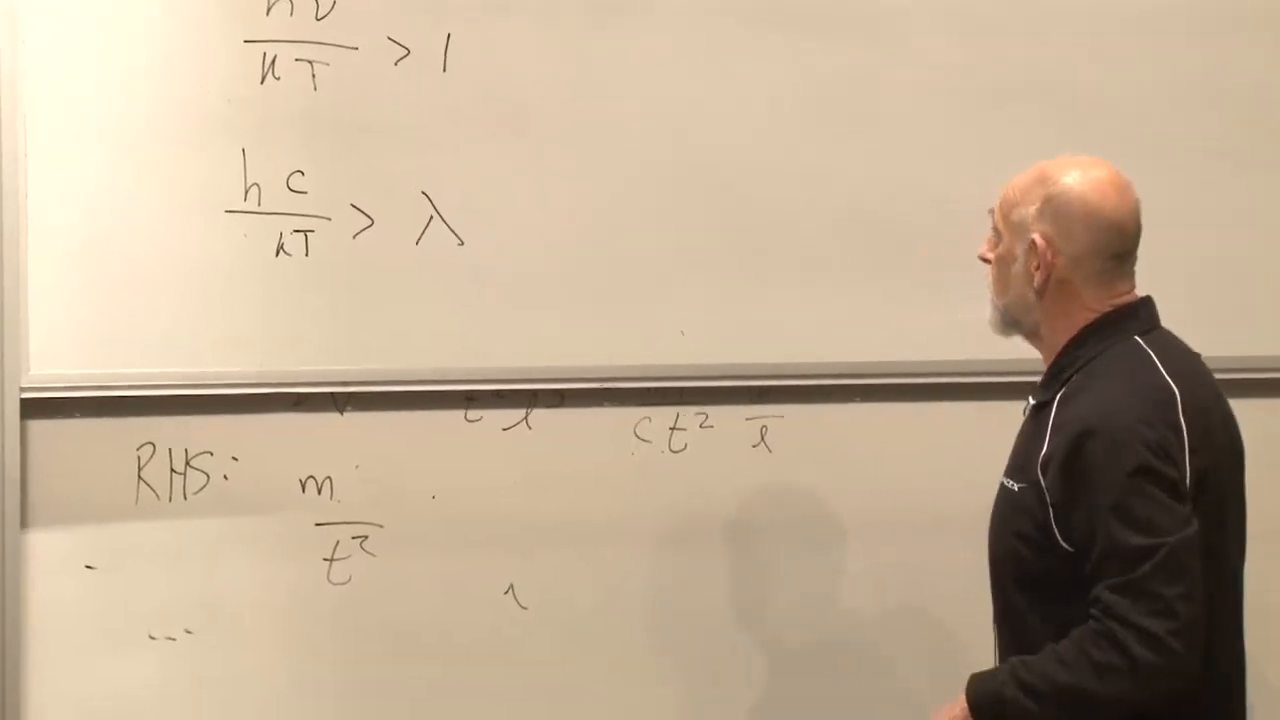
\includegraphics[width=0.82\textwidth]{lecture_07_figure_02.png}
\caption{黑板上的熱轉折。裁切後可見的上方表示式為\(h\nu/(kT)>1\)，清楚可見的下方表示式為\(hc/(kT)>\lambda\)。下方黑板上模糊的殘留內容不作為方程式的依據。}
\label{fig:c07-thermal-board}
\lectureframe{00:44:42.840}
\end{figure}

利用\(\nu=c/\lambda\)，轉折可定義一個熱波長的量級：
\begin{equation}
\boxed{\lambda_{\rm th}\sim\frac{hc}{k_BT}}.
\label{eq:c07-thermal-wavelength}
\end{equation}
更短的波長位於指數抑制的尾端；大部分功率由此量級的波長承載。具體的數值因子則取決於光譜是按單位頻率還是單位波長繪製。

\begin{classroomqa}
\audiencequestion{普朗克是用這裡採用的電子--質子等離子體模型推導出這個光譜的嗎？}
\lecturerresponse{不是。他將經驗光譜資料與維恩位移定律結合；該定律已顯示峰值波長與溫度成反比。這個尺度關係揭示了一個新的常數\(h\)。普朗克將結果與材料壁中的振子連結起來，而輻射場完整的量子詮釋則是後來才發展出來的。\lecturetimestamp{00:37:06--00:39:25}}
\end{classroomqa}

\begin{classroomqa}
\audiencequestion{為什麼量綱檢查似乎少了一個\(c\)次方？}
\lecturerresponse{最初稱為強度的量，定義為單位體積、單位頻率所含的能量；而熟悉的含有\(2h\nu^3/c^2\)的公式，指的是每單位面積、每單位立體角的譜輻射亮度。譜能量密度帶有\(c^{-3}\)及一個角度因子，如方程式~\eqref{eq:c07-planck}所示。這項修正改變的是歸一化慣例，而非無因次比值\(h\nu/(k_BT)\)或熱波長。\lecturetimestamp{00:39:33--00:44:51}}
\end{classroomqa}

除了歸一化之外，普朗克光譜具有普適形狀。方程式~\eqref{eq:c07-planck}可以寫成
\begin{equation}
u_\nu(T)=T^3\,F\!\left(\frac{\nu}{T}\right),
\label{eq:c07-scaling-form}
\end{equation}
其中常數都吸收到\(F\)中。提高\(T\)會重新縮放頻率軸與整體高度，但無因次曲線的形狀不變。以波長來說，溫度升高會使光譜往較短波長方向收縮。

\begin{figure}[htbp]
\centering
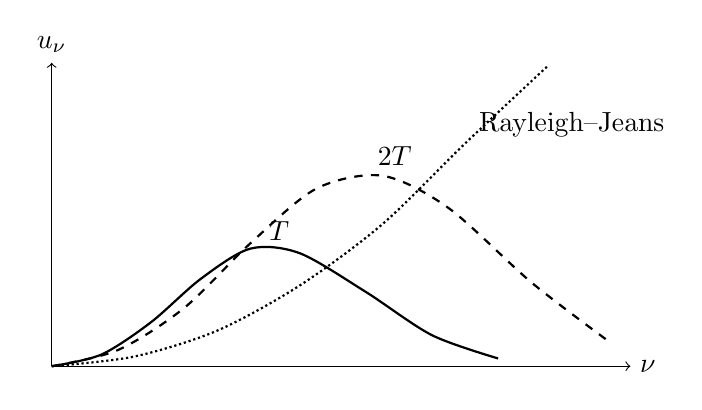
\begin{tikzpicture}[x=1.05cm,y=0.82cm]
\draw[->] (0,0)--(7.0,0) node[right] {\(\nu\)};
\draw[->] (0,0)--(0,4.7) node[above] {\(u_\nu\)};
\draw[densely dotted,thick] plot[smooth] coordinates
  {(0,0) (1,0.15) (2,0.55) (3,1.25) (4,2.20) (5,3.45) (6,4.65)};
\draw[thick] plot[smooth] coordinates
  {(0,0) (0.6,0.18) (1.2,0.68) (1.8,1.35) (2.4,1.82) (3.0,1.75) (3.8,1.15) (4.6,0.48) (5.4,0.12)};
\draw[thick,dashed] plot[smooth] coordinates
  {(0,0) (0.8,0.25) (1.6,0.90) (2.4,1.90) (3.2,2.75) (4.0,2.95) (4.8,2.45) (5.8,1.30) (6.7,0.42)};
\node[anchor=west] at (5.05,3.75) {Rayleigh--Jeans};
\node at (2.75,2.10) {\(T\)};
\node at (4.15,3.25) {\(2T\)};
\end{tikzpicture}
\caption{經典光譜無限制地上升，普朗克光譜則會轉折。溫度升高會使特徵頻率往高頻移動，同時維持無因次形狀不變。}
\label{fig:c07-planck-redraw}
\end{figure}

當今宇宙中絕大多數光子都屬於微波背景，其特徵波長約為毫米量級。方程式~\eqref{eq:c07-thermal-wavelength}將這個波長與數克耳文的溫度相聯繫，此處依慣例取整為\(3\,\mathrm{K}\)。單憑波長只能粗略推知溫度。更有力的證據是，不同頻率的測量以極高精度描繪出完整的黑體曲線。

\begin{classroomqa}
\audiencequestion{一個微波背景光子占據多大的空間？}
\lecturerresponse{光子沒有普遍適用、邊界分明的尺寸。光子可以被製備成波包，其空間展布取決於狀態；波長則設定了振盪的尺度。對熱背景而言，特徵波長與自然的波包尺度都在毫米量級，但兩者都不應被誤認為小型經典物體的半徑。\lecturetimestamp{00:57:16--00:59:05}}
\end{classroomqa}

\section{膨脹凍結了黑體形狀}

先從一個充滿電離氫與平衡輻射的熱盒子開始。盒子膨脹時，其中的物質對外做功，能量密度下降，溫度也降低。最後，電子與質子維持束縛狀態，形成中性原子。原子形成的過程稱為\emph{復合}；光子--物質散射效率降低的過程稱為\emph{退耦}。兩個過程密切相關，但指的是不同的物理事件。

退耦之後，物質與輻射不再共享同一溫度，但光子光譜仍保持普朗克形式。每個自由傳播的波長都受到相同膨脹因子的拉伸，
\begin{equation}
\lambda\propto a,
\qquad
\nu\propto a^{-1}.
\end{equation}
由於普朗克曲線取決於\(\nu/T\)，這種均勻紅移等效於為輻射指定一個溫度
\begin{equation}
\boxed{T_\gamma\propto a^{-1}.}
\label{eq:c07-temperature-scaling}
\end{equation}
因此，即使沒有碰撞持續重建光譜，膨脹仍能維持其形狀。物質則遵循自身後續的熱史。

因此，觀測到的微波背景是平衡分布留下的化石。自由電荷有效散射時，黑體形式便已建立；之後，它隨均勻的宇宙學紅移一路演化至今。星光、伽馬射線及其他較晚出現的來源也都存在，但與遺留光子族群相比，數量少得多，而且各有可辨認的天體物理起源。

\begin{classroomqa}
\audiencequestion{輻射不再與物質處於平衡後，為何仍能保持黑體形狀？}
\lecturerresponse{碰撞是形成平衡光譜所必需的，但若膨脹完全均勻，維持光譜形狀就不需要碰撞。每個波長都乘上相同因子，會將一個普朗克光譜轉換成另一個溫度較低的普朗克光譜。光子不再與物質共享溫度，但仍有自身的黑體溫度。}
\end{classroomqa}

\section{為何復合發生得如此晚}

今天的波長與退耦時的波長之間，關係如下：
\begin{equation}
\frac{\lambda_0}{\lambda_{\rm dec}}
=
\frac{a_0}{a_{\rm dec}}
=
\frac{T_{\rm dec}}{T_0}.
\label{eq:c07-decoupling-ratio}
\end{equation}
退耦在數學上並非瞬時發生，但相較於後續宇宙史，這個過程短暫得足以指定一個特徵尺度因子與溫度。此處的\(T_0\)指的是CMB溫度，而非星系際物質的動力學溫度。

氫基態的電離能為
\begin{equation}
\chi_H=13.6\,\mathrm{eV}.
\end{equation}
直覺上會先猜\(k_BT\sim\chi_H\)，如此一來，一個典型光子便能電離一個原子。但這個估計的溫度高出許多，因為熱光譜具有高能尾端，而且宇宙中的光子數量極其龐大。

\begin{figure}[htbp]
\centering
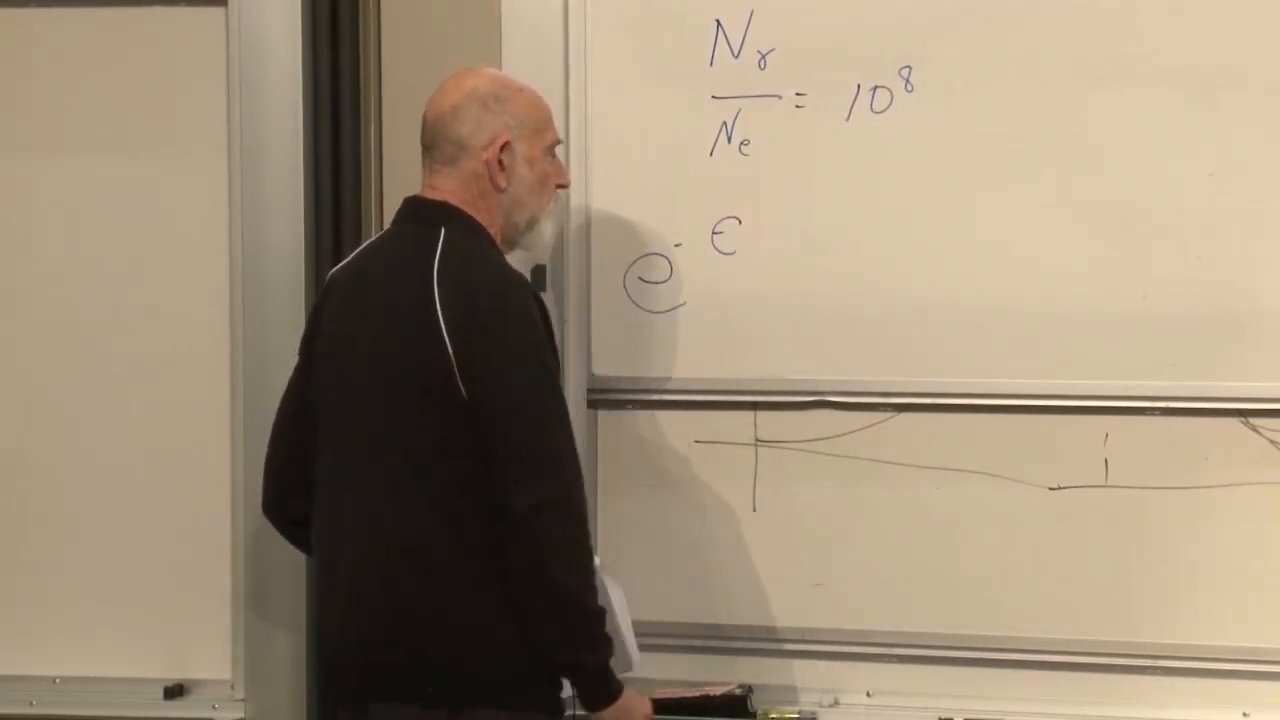
\includegraphics[width=0.82\textwidth]{lecture_07_figure_03.png}
\caption{黑板上引入了觀測到的豐度比\(N_\gamma/N_e=10^8\)與光子能量符號\(\epsilon\)。圖中只能看到指數項的開頭部分；完整的波茲曼因子是從口頭推導得出的。}
\label{fig:c07-boltzmann-board}
\lectureframe{01:06:10.631}
\end{figure}

此處採用的豐度比約值為
\begin{equation}
\frac{N_\gamma}{N_e}\sim10^8.
\label{eq:c07-photon-electron-ratio}
\end{equation}
此值是比較測得的CMB光子密度與普通物質總量後推得的。對能量為\(\epsilon\)的光子，高能尾端具有波茲曼形式
\begin{equation}
P(\epsilon)\propto e^{-\epsilon/(k_BT)}.
\end{equation}
因此，每個原子可取得的電離光子數估計為
\begin{equation}
10^8 e^{-\chi_H/(k_BT)}.
\end{equation}
直到這個數量降至約為一時，電離仍然有效。

取對數可得
\begin{equation}
\frac{\chi_H}{k_BT}
\sim
\ln 10^8
\simeq18.4,
\end{equation}
或者，以所需的精確度表示，
\begin{equation}
k_BT\sim\frac{\chi_H}{20}.
\label{eq:c07-tail-estimate}
\end{equation}
特徵光子的能量可以遠低於電離閾值，因為每個原子只要有一個來自尾端的電離光子便足夠。

\begin{classroomqa}
\audiencequestion{尾端估計計算的是恰好位於閾值的光子，還是所有能量高於閾值的光子？}
\lecturerresponse{計算的是能量等於或高於閾值的光子。由於尾端按指數衰減，積分的大部分來自能量接近\(\chi_H\)的光子，因此簡單的指數估計足以掌握相關的量級。\lecturetimestamp{01:08:39--01:08:54}}
\end{classroomqa}

\begin{classroomqa}
\audiencequestion{在退耦時，比值\(N_\gamma/N_e\)也約為\(10^8\)嗎？}
\lecturerresponse{以此處採用的近似而言，是的。從退耦回溯到溫度高得多的時期，膨脹以相同的體積因子稀釋這兩種粒子族群；而且，兩者都沒有產生或消滅到足以改變其比值的程度。到了更高溫時，對產生反應就需要另行計算。\lecturetimestamp{01:08:54--01:09:57}}
\end{classroomqa}

\begin{classroomqa}
\audiencequestion{恆星發出的光子對這項計數有顯著貢獻嗎？}
\lecturerresponse{沒有。復合時期尚未有恆星形成，即使到了今天，恆星光子相較於CMB光子族群仍只占極小一部分。方程式~\eqref{eq:c07-photon-electron-ratio}中的比值指的是遺留的熱光子。\lecturetimestamp{01:11:44--01:12:39}}
\end{classroomqa}

\begin{classroomqa}
\audiencequestion{電子與質子復合時所放出的光子，是否應在黑體光譜中留下明顯的氫譜線？}
\lecturerresponse{只要散射與吸收相對於膨脹仍然夠快，輻射就會持續重新處理，並維持接近熱平衡。若凍結過程足夠突然，確實可能留下光譜畸變；但復合過程緩慢且接近平衡，因此不會留下足以取代黑體形式的強烈孤立譜線。\lecturetimestamp{01:12:42--01:14:07}}
\end{classroomqa}

課堂上的估計結果是\(T_{\rm dec}\sim4\times10^3\,\mathrm{K}\)。直接將\(\chi_H/20\)換算成溫度，會得到略高的數值，因此有效分母可能更接近\(40\)。這並不矛盾，而是顯示用一次尾端計數取代完整電離平衡有多粗略。若要進行受控的平衡計算，需使用薩哈關係，
\begin{equation}
\frac{x_e^2}{1-x_e}
=
\frac{1}{n_H}
\left(\frac{m_e k_BT}{2\pi\hbar^2}\right)^{3/2}
e^{-\chi_H/(k_BT)},
\label{eq:c07-saha}
\end{equation}
接著再考慮非平衡復合動力學。這項粗略論證的價值，在於指出主導物理：極小的重子與光子比，讓中性原子要到遠低於\(\chi_H/k_B\)的溫度才得以存留。

\section{紅移至最後散射面}

取\(T_0\simeq3\,\mathrm{K}\)和\(T_{\rm dec}\sim4\times10^3\,\mathrm{K}\)，由方程式~\eqref{eq:c07-decoupling-ratio}可得
\begin{equation}
\boxed{
\frac{a_0}{a_{\rm dec}}
\sim
\frac{T_{\rm dec}}{T_0}
\sim10^3
}.
\label{eq:c07-decoupling-expansion}
\end{equation}
同樣地，最後散射紅移的量級為\(10^3\)。在此時期之前，電離等離子體是不透明的；此後光子便近乎自由地傳播。

這個熱事件發生在熱膨脹開始後僅幾十萬年；課堂對話中通常約記為\(380{,}000\)年。相較於此後的宇宙年齡，這段時間極短。自退耦以來，長度增加了約\(10^3\)倍，共動體積元素則增加了約\(10^9\)倍。

退耦是熱史上的一個里程碑，卻不是這段期間唯一的事件。星系、恆星與黑洞都在更晚時期形成；此處先不討論它們，讓我們能清楚回溯各個熱史里程碑。

望向遠方，就是望向過去。近處的殼層呈現較近的時期，較遠處的殼層則呈現更早的時期。我們的過去光錐最終與復合時期相交；兩者的交集就是最後散射面。更早期的電磁輻射反覆受到自由電荷散射，無法直接傳到我們這裡。

\begin{figure}[htbp]
\centering
\begin{coursefitfigure}
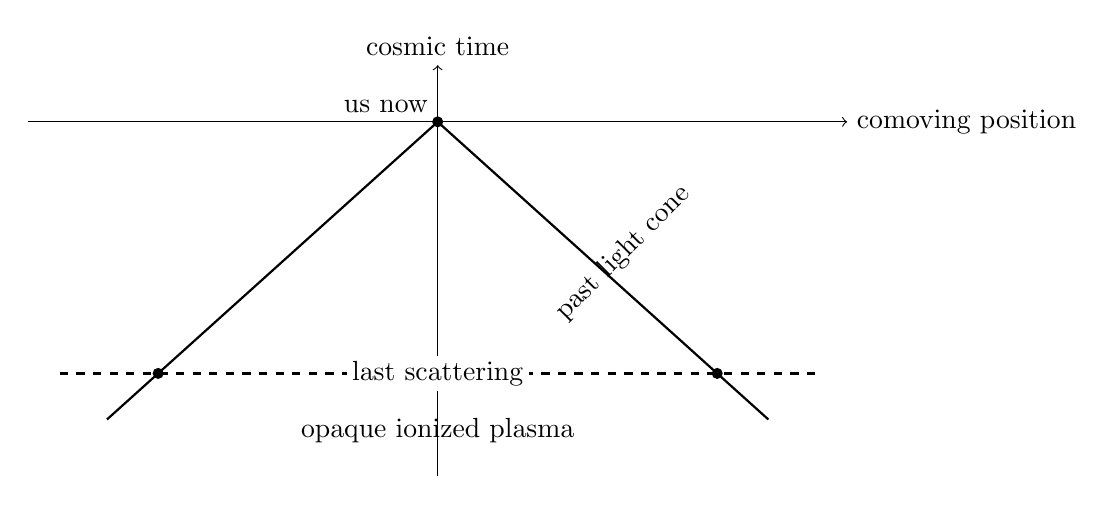
\begin{tikzpicture}[x=1.0cm,y=0.9cm]
\draw[->] (0,0)--(0,5.8) node[above] {cosmic time};
\draw[->] (-5.2,5.0)--(5.2,5.0) node[right] {comoving position};
\draw[thick] (0,5.0)--(-4.2,0.8);
\draw[thick] (0,5.0)--(4.2,0.8);
\draw[thick,dashed] (-4.8,1.45)--(4.8,1.45);
\fill (0,5.0) circle (2pt) node[above left] {us now};
\fill (-3.55,1.45) circle (2pt);
\fill (3.55,1.45) circle (2pt);
\node[fill=white,inner sep=2pt] at (0,1.45) {last scattering};
\node at (0,0.65) {opaque ionized plasma};
\node[rotate=45] at (2.35,3.15) {past light cone};
\end{tikzpicture}
\end{coursefitfigure}
\caption{電磁觀測沿著過去光錐回溯，最遠只能到達最後散射面。更早期的光子曾在電離等離子體中反覆散射。}
\label{fig:c07-last-scattering}
\end{figure}

\begin{classroomqa}
\audiencequestion{退耦是否讓我們無法以任何方式觀測更早的時期？}
\lecturerresponse{它使我們無法直接以電磁方式觀測，因為等離子體對光子不透明。相互作用較弱的信使能從更早期逃逸：遺留中微子原則上可探測更早的一層，而重力波則能攜帶更早時期的資訊。因此，我們對最後散射之前的認識大多是間接的，但並非毫無根據。\lecturetimestamp{01:32:27--01:36:31}}
\end{classroomqa}

\begin{classroomqa}
\audiencequestion{\(a\)在宇宙開端時的絕對值是多少？宇宙必然是微小而有限的物體嗎？}
\lecturerresponse{在平坦空間中，只有尺度因子之比具有不變的意義；\(a\)的歸一化可以任意選取。負曲率的空間切片也可能是無限大的。封閉的\(k=+1\)宇宙具有有限的曲率半徑，但觀測所能確定的仍是膨脹比，而非已知的原初大小。熱大爆炸本身並不表示所有空間曾是一個微小球體。\lecturetimestamp{01:30:05--01:32:22}}
\end{classroomqa}

\begin{classroomqa}
\audiencequestion{CMB比星系古老；觀測到CMB是否能告訴我們，在今日可觀測區域之外是否也有星系？}
\lecturerresponse{不能。CMB呈現的是遙遠區域在退耦時的狀態，而非該區域的現況。來自足夠遙遠、今日已存在的星系的光，還沒有足夠時間抵達我們。支持視界之外仍有星系族群的，是觀測到的大尺度均勻性與看不到明確邊界，而非CMB提供的直接觀測。\lecturetimestamp{01:59:01--02:00:58}}
\end{classroomqa}

時間線由現在往回追溯，經過星系形成與退耦，直到物質--輻射相等。再往前，尺度因子愈小，溫度愈高，也會出現新的粒子種類。

\section{物質--輻射相等}

越過退耦繼續回溯，會遇到另一個里程碑。非相對論性物質與輻射的稀釋方式不同：
\begin{equation}
\rho_m\propto a^{-3},
\qquad
\rho_r\propto a^{-4},
\qquad
\frac{\rho_m}{\rho_r}\propto a.
\label{eq:c07-equality-scaling}
\end{equation}
晚期由物質主導，但當\(a\)小到一定程度時，輻射必然占主導地位。膨脹定律也相應地從物質主導時期的行為\(a\propto t^{2/3}\)轉為輻射主導時期的行為\(a\propto t^{1/2}\)。

一個刻意簡化的粗略估計，從每個質子\(10^8\)個光子、CMB光子的特徵能量\(10^{-4}\,\mathrm{eV}\)及質子的靜止能量\(10^9\,\mathrm{eV}\)出發。忽略暗物質可得
\begin{equation}
\left(\frac{\rho_m}{\rho_r}\right)_0
\sim
\frac{10^9}{10^8\,10^{-4}}
\sim10^5.
\end{equation}
接著修正這項估計：暗物質的質量遠高於發光重子，將取整後的估計提高至\(10^6\)。依據這項計算，方程式~\eqref{eq:c07-equality-scaling}給出的相等時期為
\begin{equation}
\frac{a_{\rm eq}}{a_0}\sim10^{-6},
\qquad
\frac{T_{\rm eq}}{T_0}\sim10^6.
\label{eq:c07-equality-estimate}
\end{equation}
這些是用來估定尺度的課堂粗略估計，並非精確的宇宙學參數擬合。其目的是展示\(a\)的不同冪次如何定位各個接續的熱時期。

輻射主導時期位於電磁觀測所能抵達的最後散射界線之前，但根據測得的晚期密度與已知標度律，仍可推知它確實存在。溫度繼續升高後，質子、電子與光子數目各自固定的假設終將失效，因為高能碰撞會開始產生大質量粒子--反粒子對。

\begin{classroomqa}
\audiencequestion{光子數與質子數守恆的說法，是否也涵蓋星光與任意高的溫度？}
\lecturerresponse{不。這個說法適用於殘留CMB光子族群，且僅限於改變粒子數的反應不起作用的時期。星光是後來才產生的，在光子計數中可以忽略。溫度足夠高時，對產生會改變粒子組成，個別粒子數便不再守恆。復合本身至多每個電子增加約一個光子，僅占現有CMB光子族群的\(10^8\)分之一。\lecturetimestamp{01:26:24--01:27:40}}
\end{classroomqa}

\section{對產生與幾乎對稱的原始湯}

溫度約為
\begin{equation}
T\sim10^{10}\,\mathrm{K},
\qquad
\frac{a_0}{a}\sim10^{14},
\end{equation}
時，特徵光子能量約為一百萬電子伏特，與產生電子--正電子對所需的靜止能量尺度相當。此時兩個光子可以透過下列反應
\begin{equation}
\gamma+\gamma
\longleftrightarrow
e^-+e^+.
\label{eq:c07-pair-reaction}
\end{equation}
互相轉換。精確閾值取決於碰撞運動學，但電子靜止能量\(m_ec^2\)決定了相關尺度。

對產生與對湮滅會迅速達到平衡。若對的數量太少，光子碰撞會補充它們；若對的數量太多，湮滅便會將其能量還給光子。因此，在相對論性等離子體中，光子、電子與正電子的豐度都由溫度決定，且量級相近。它們不再簡單地保留日後粒子數量的資訊。

\begin{classroomqa}
\audiencequestion{如果已有電子用來平衡質子的電荷，充滿粒子對的等離子體如何仍能保持電中性？}
\lecturerresponse{每次反應都會產生一個負電荷與一個正電荷，因此粒子對不會增加淨電荷。大量近乎對稱的粒子族群，疊加在微小的電子過量之上。各個電子彼此不可區分；只有差值\(N_{e^-}-N_{e^+}\)保留了平衡質子所需的電荷資訊。\lecturetimestamp{01:42:31--01:43:14}}
\end{classroomqa}

粒子對反應會改變總和，但差值保持不變：
\begin{equation}
N_{e^-}+N_{e^+}\quad\hbox{changes},
\qquad
N_{e^-}-N_{e^+}=\hbox{constant}.
\label{eq:c07-pair-invariants}
\end{equation}
在熱湯中，\(N_{e^-}+N_{e^+}\)與\(N_\gamma\)的量級相近；留下的過量則與數量小得多的質子相當。因此，取整後的比值為
\begin{equation}
\boxed{
\frac{N_{e^-}-N_{e^+}}
{N_{e^-}+N_{e^+}}
\sim10^{-8}
}.
\label{eq:c07-asymmetry}
\end{equation}
約每\(10^8\)個電子--正電子對，就有一個過量電子。

這使我們反過來看待最初的問題。引人注目的不只是光子數量龐大；在高溫下，光子與粒子對自然具有相近的豐度。真正的謎題是，為何負粒子與正粒子的數量會有差異，以及為何相對差異如此微小，而非恰好為零或達到一的量級。對稱的初始狀態加上對稱的粒子對產生，理應不會留下任何過量。非零不對稱性的微觀起源，就是接下來要探討的問題。

溫度再高出兩、三個數量級時，便不能再忽略質子結構。碰撞會產生夸克與反夸克，質子也會解離成其組成粒子；光子、輕子、夸克、反夸克、膠子，以及任何質量足夠低的暗物質粒子，共同構成更熱的等離子體。此時真空能在動力學上可忽略，因為輻射密度按\(a^{-4}\)增長。

夸克的過剩量透過整體電荷中性，與電子的過剩量相互關聯。三個價夸克構成一個重子，因此依慣例，兩者的數量核算相差一個因子；但殘存的重子物質與殘存的電子，並非彼此獨立的電荷不平衡。它們共同的微小性，是早期宇宙留下的遺跡。

再來追溯電子--正電子電漿的演化。溫度一旦降到粒子對產生的能量尺度以下，湮滅便持續進行，逆反應則日漸稀少。幾乎每個電子都會找到一個正電子，粒子對的能量轉化為輻射，只剩下極少數未配對的電子。我們周遭的物質，正是這種殘餘的不平衡，而不是曾經數量龐大的粒子對的代表性樣本。

\begin{classroomqa}
\audiencequestion{在電子--正電子湮滅的時期，質子在做什麼？}
\lecturerresponse{當時的溫度足以產生電子對，但還不足以大量產生質子--反質子對，也不足以使質子解離成夸克。因此，質子數量雖少，卻持續存在；為了維持電中性，必須有 \(N_{e^-}-N_{e^+}\simeq N_p\)。 \lecturetimestamp{01:55:35--01:56:53}}
\end{classroomqa}

可見宇宙中的物質過剩似乎處處同號。課堂上提出的證據，是宇宙射線中沒有反原子核：次級碰撞偶爾會產生反質子，但若有反星系，預期便會有複雜的反原子核。這是當時講課所採用的觀測論據，並不表示已經觀測過可觀測視界以外的區域。

\begin{classroomqa}
\audiencequestion{觀測到的物質過剩會不會只是局部漲落，而我們看不到的地方其實存在反物質區域？}
\lecturerresponse{在如此巨大的可觀測體積內，物質過剩同號，這種一致性遠非隨機漲落所能解釋，必須有動力學上的解釋。然而，可觀測區域之外沒有直接證據；不能僅因我們觀測到的範圍已超出光所能到達之處，就排除存在不同區域的可能性。 \lecturetimestamp{01:56:57--01:58:47}}
\end{classroomqa}

\begin{classroomqa}
\audiencequestion{物質--反物質的解釋已經是精確的數值理論了嗎？力的統一會在這個溫度下發生嗎？}
\lecturerresponse{目前已有一套定性理論，說明微小的不對稱性可能如何形成；但此處並未從某個唯一的微觀模型推導出經過取整的 \(10^{-8}\) 數值。力的統一發生於遠高於電子對形成時期的溫度。這兩個問題都需要探討目前列出的熱歷史基準之外的物理。 \lecturetimestamp{01:51:36--01:52:24}}
\end{classroomqa}

\section{本節要點}

熱歷史由反應速率與閾值所決定。快速散射使各成分維持共同溫度；中性原子形成後，散射粒子隨之消失；接著，宇宙均勻膨脹使凍結的普朗克譜發生紅移，但不改變其形狀。因此，宇宙微波背景（CMB）既是輻射的溫度計，也是標示電磁波無法再直接探測更早期電漿的可見表面。

光子過剩使再結合成為由高能尾端主導的問題，而非由平均能量主導。尺度\(T_{\rm dec}/T_0\sim10^3\)標示了末次散射發生的時期；物質與輻射各自不同的稀釋規律，則標示出更早的物質輻射相等時期。溫度再升高時，粒子對的產生會抹去電子與正電子總數的記憶，卻保留兩者之間的微小差值。重子部分也有相應的殘餘不對稱性；這項尚未解釋的初始條件，是接下來必須面對的問題。
